\chapter{Analýza}
%% Analýza a návrh implementace (včetně diskuse různých alternativ a volby implementačního prostředí).

%% V části analýzy provést rozbor jednotlivých principů + výsledky rešerší - využívat hojně informace z článků a důsledně citovat zdroje

\section{Analýza principů objektového návrhu}

%% PRINCIPY versus PATTERNY -> citovat clanek

\subsection{Analyzované principy}
Ukázkové návrhové principy analyzované v rámci této práce jsou znázorněny na obrázku \ref{analyzed_principles}. Poznamenejme, že tzv. Demeterův zákon je speciálním případem pravidla pro \uv{low coupling}.

\begin{figure}[h!]
\centering
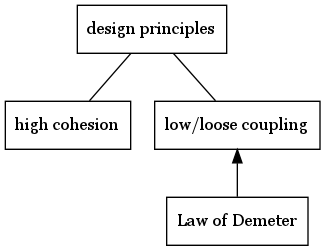
\includegraphics[width=0.5\textwidth]{./graphs/oop_design_principles.png}
\caption{Znázornění analyzovaných návrhových principů.\label{analyzed_principles}}
\end{figure}

% TODO: v rámci každého návrhového principu uvést příklad porušení
% tohoto principu (případně i příklad, který tento princip dodržuje)

% Příklad pravidla:
% ``Třídy z balíčku A nesmí záviset na jiných konkrétních třídách, ale nejvýše na rozhraních balícků B.''
%  (programování proti rozhraní namísto proti kokrétní implementaci)"

\subsubsection{Low coupling}

\subsubsection{High cohesion}

\subsubsection{Law of Demeter}

Existuje několik forem Demeterova zákona \cite{35588}, které jsou vhodné pro různé oblasti aplikace. Tyto typy jsou znázorněny na obrázku \ref{demeter_law_types}.

\begin{figure}[h!]
\centering
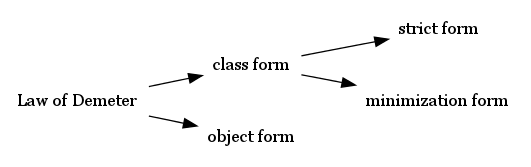
\includegraphics[width=0.7\textwidth]{./graphs/demeter_law_types.png}
\caption{Formy Demeterova zákona.\label{demeter_law_types}}
\end{figure}

Pro statickou analýzu lze použít \uv{class} formu Demeterova zákona.

\subsection{Ukázky kódu porušujících některá z pravidel}

\subsubsection{Porušení principu law of Demeter}

%% TODO: use some highlighter
%% TODO: add example of demeter law violation from paper notes
\begin{verbatim}
package handlers;

public class ...

\end{verbatim}

\section{Analýza problematiky v jazyce Java}

\subsection{Statický model programu v Javě}
% TODO: provide better name for this section
\subsubsection{Struktura Java projektu}

\subsubsection{Základní syntaktické elementy programovacího jazyka Java}
Grafické znázornění základních syntaktických elementů, jejichž struktura a názvy jsou převzaty z \cite{Gosling:2005:JLS:1036643}, je na obrázku \ref{toplevel_elements}.
% TODO: write some better accompanying text
\begin{figure}[h!]
\centering
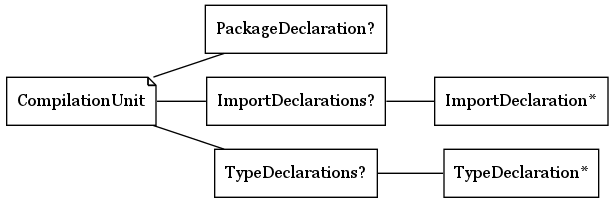
\includegraphics[width=\textwidth]{./graphs/java_top_elements.png}
\caption{Struktura základních syntaktických elementů programovacího jazyka Java.\label{toplevel_elements}}
\end{figure}

Pro analýzu založenou na vyhledávání závislostí mezi třídami pro nás bude nejdůležitější syntaktický element \emph{TypeDeclaration}. Tento neterminální symbol se dále přepisuje na symboly uvedené na obrázku \ref{type_declaration_options}.

\begin{figure}[h!]
\centering
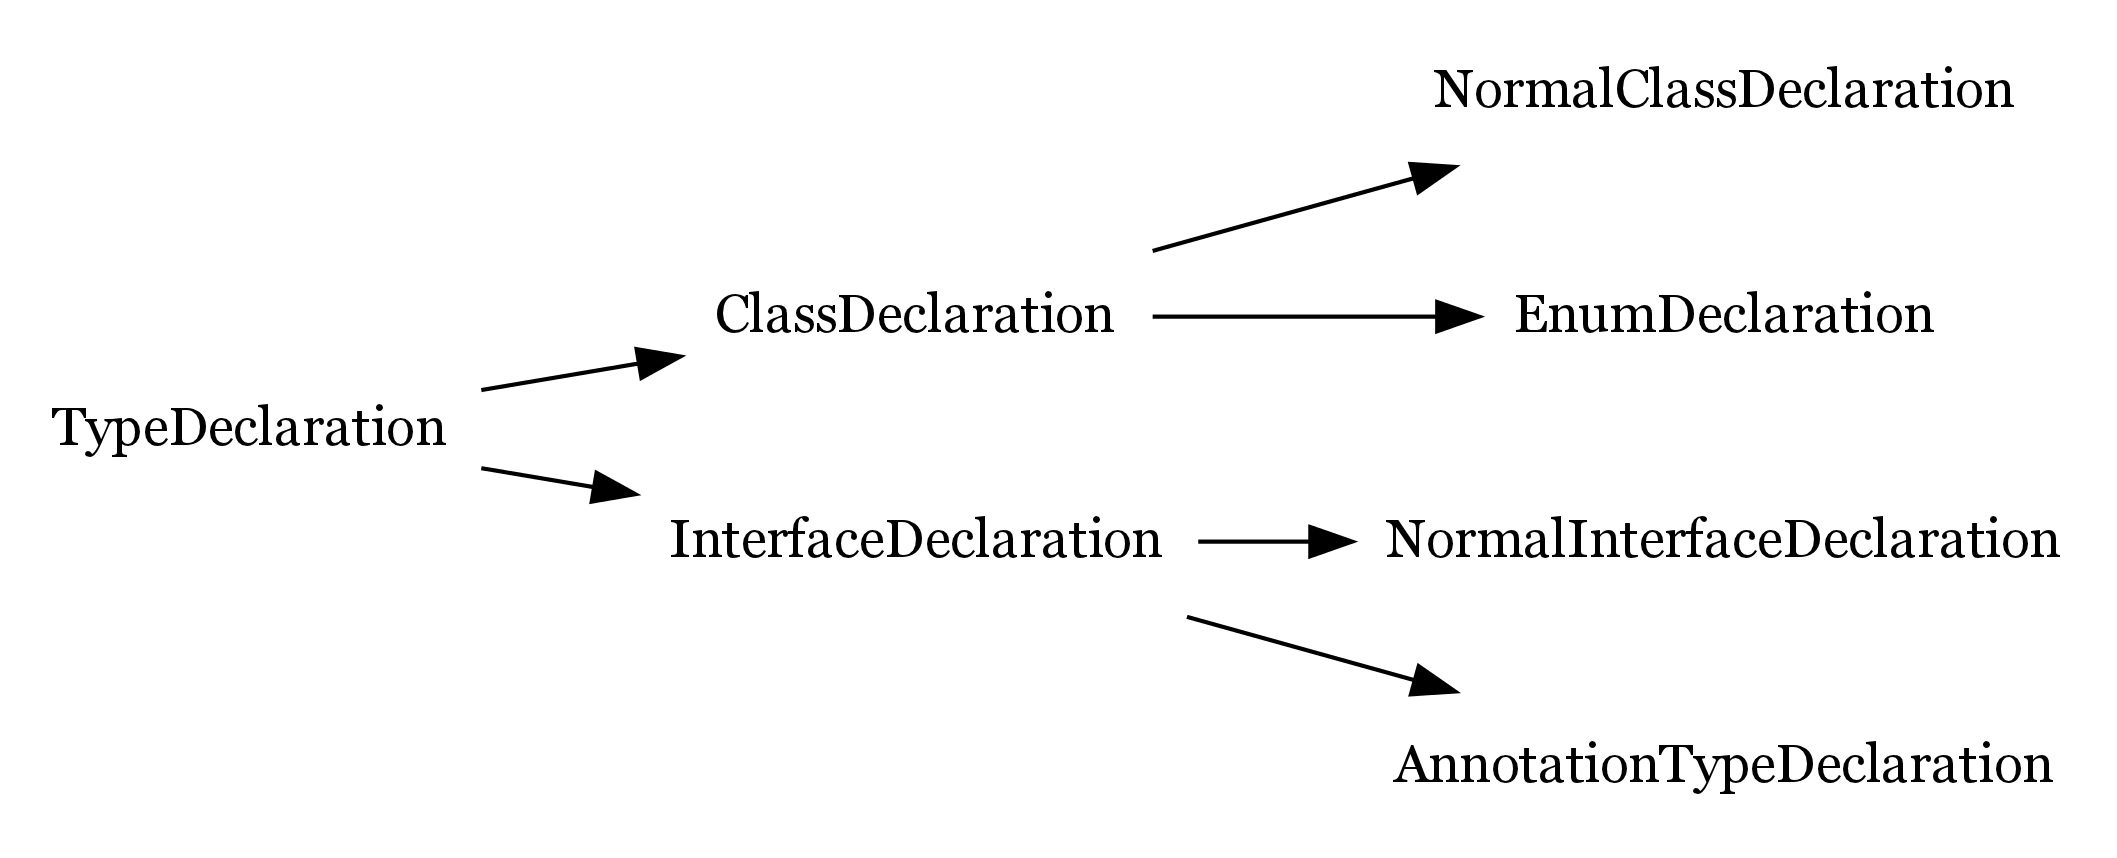
\includegraphics[width=\textwidth]{./graphs/toplevel_types.png}
\caption{Rozklad elementu TypeDeclaration.\label{type_declaration_options}}
\end{figure}

\section{Existující nástroje pro statickou analýzu kódu v Javě}
% TODO: add some background research on existing tools (take information from wiki, ../materials)
